\documentclass[11pt]{article}

\input{Shared.tex}

\parindent0in
\pagestyle{plain}
\thispagestyle{plain}

\usepackage{csquotes}
\usepackage[shortlabels]{enumitem}

\newcommand{\dated}{\today}
\newcommand{\token}[1]{\langle \text{#1} \rangle}

\begin{document}

\textbf{Introduction to the Theory of
Computation}\hfill\textbf{\myname}\\[0.01in]
\textbf{Chapter 8: Space Complexity}\hfill\textbf{\dated}\\
\smallskip\hrule\bigskip

\begin{problem}{8.25}
An undirected graph is \textbf{\textit{bipartite}} if its nodes may be divided into two sets so that all edges go from a node in one set to a node in the other set. Show that a graph is bipartite if and only if it doesn't contain a cycle that has an odd number of nodes. Let $BIPARTITE = \{\langle G \rangle \ | \ G \text{ is a bipartite graph}\}$. Show that $BIPARTITE \in $ NL.
\end{problem}

\begin{problem}[Part]{a}
Show that an undirected graph is bipartite if and only if it doesn't contain a cycle that has an odd number of nodes.
\end{problem}

\begin{proof}
For the forward direction, let $G$ be a bipartite graph and show that $G$ doesn't contain a cycle that has an odd number of nodes. The proof is by contradiction. Assume that $G$ contains a a cycle $n_1, n_2, \ldots , n_{k-1}, n_k$ that has an odd number of nodes. Then, it must be the case that nodes $n_1$ and $n_{k-1}$ are assigned to different sets because every two consecutive nodes in the sequence $n_1, n_2, \ldots , n_{k-1}, n_k$ are adjacent to each other. But this implies that node $n_k$ cannot be assigned to either first or second set as it is adjacent to both nodes $n_1$ and $n_{k-1}$, which is a contradiction. \\

To prove the other direction of the theorem, let $G$ be an undirected graph that doesn't contain a cycle that has an odd number of nodes and show that $G$ is bipartite. The proof is by contradiction. Assume that $G$ is not bipartite. Then, there must exist three nodes $u$, $v$ and $w$, such that nodes $u$ and $v$ must be belong to different sets and node $w$ is adjacent to both $u$ and $v$. This implies that, a path  from $u$ to $v$ exists that contains an even number of nodes, and path from $u$ to $w$ is a cycle that has an odd number of nodes, which is a contradiction.
\begin{center}
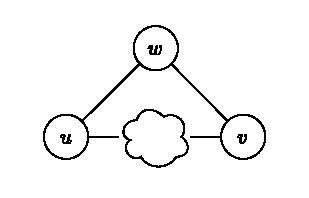
\includegraphics[scale=1.0]{Figures/Problem8.25.pdf}
\end{center}
\end{proof}

\begin{problem}[Part]{b}
Show that $BIPARTITE \in $ NL.
\end{problem}

\begin{proof}
\end{proof}

\end{document}